\chapter{Voting and Mechanism Design}

Once you have a multiagent system composed of autonomous locally-aware
agents, you will often desire a way to aggregate their knowledge for
making a system-wide decision. That is, you will want to ask them to
vote on some issue. Unfortunately, there are many different voting
mechanisms, each one of which might lead to different answers. More
importantly, it could be that selfish agents do not want to vote their
true preferences. They might prefer to lie, in the same way you might
not vote for your favorite political candidate if you think that she
does not have any hope of winning and, instead, you vote for your
second most favorite candidate. In this chapter we examine the
problems with voting and mechanism design.

\section{The Voting Problem}
\label{sec:voting-problem}

At first glance, the voting problem seems very simple. We ask all
agents to proclaim their preferences over a set of candidates and then
tally these votes to find the most preferred candidate.  The problem
comes if we want this result to match, in some way, the agents'
preferences. It turns out that the common voting mechanisms all fail
to aggregate the voters' preferences in some cases.

\begin{SCfigure}
  \begin{minipage}{1.0\linewidth}
    \begin{center}
      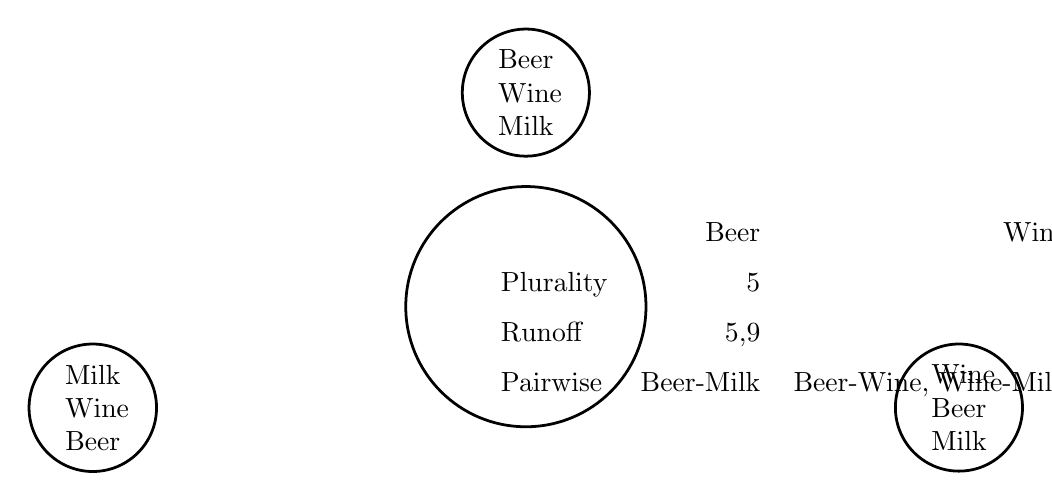
\begin{tikzpicture}[line width=1pt]
        \person{(-6,-1)}
        \person{(-6,-2)}
        \person{(-6,0)}
        \person{(-5,-1)}
        \person{(-5,-2)}
        \person{(-5,0)}

        \person{(-1,3)}
        \person{(0,3)}
        \person{(1,3)}
        \person{(-.5,2)}
        \person{(.5,2)}

        \person{(5,-1)}
        \person{(5,-2)}
        \person{(6,-1)}
        \person{(6,-2)}

        \node at (-5.5,-3)[anchor=north,text width=2em]
        {Milk\\ Wine \\Beer};

        \node at (5.5,-3)[anchor=north,text width=2em]
        {Wine \\Beer\\ Milk};

        \node at (0,1)[anchor=north, text width=2em]
        {Beer\\ Wine \\Milk};

        \node at (0,-1)[anchor=north] {
          \begin{tabular}{lrrr} \toprule
            & Beer & Wine & Milk \\ \midrule
            Plurality & 5 & 4 & 6 \\ 
            Runoff & 5,9 & 4 & 6,6 \\ 
            Pairwise & Beer-Milk & Beer-Wine, Wine-Milk & 0 \\ \bottomrule
          \end{tabular}};
      \end{tikzpicture}
    \end{center}
  \end{minipage}
  \caption{Fifteen mathematicians trying to decide whether they should buy beer, wine, or milk.}
  \label{fig:voters}
\end{SCfigure}

For example, figure~\ref{fig:voters} shows 15 mathematicians who are
planning to throw a party. They must first decide which beverage the
math department will serve at this party. There are three choices
available to them: beer, wine, and milk. As the figure shows, 6
mathematicians prefer milk over wine and wine over beer, 5 prefer beer
over wine and wine over milk and 4 prefer wine over beer and beer over
milk.  We then need to determine which drink they will choose.

One option is to have a \td{plurality vote} where each one votes for
their favorite drink, the votes are tallied and the drink with the
most votes is the winner. Under this voting scheme beer would get 5
votes, wine 4, and milk 6. Therefore, the mathematicians should
clearly choose milk as the drink for the party.

Another option is to have a \td{runoff} election (primaries) then
pick the two winners and have another election with only those two
(these technique can be easily extended to any number of runoff
elections). Under this scheme the first election would lead to the
same votes as before so the second election would consist of beer and
milk. With only these two candidates beer would get 9 votes while milk
would get 6 votes. Therefore, the mathematicians should clearly choose
beer as the drink for the party.

Yet another option is to hold three elections each one with only two
candidates (that is, implement all \td{pairwise} elections) and the
candidate that wins the most elections is the chosen one. Under this
scheme we would see that if beer and wine are paired then wine wins,
if beer and milk are paired then beer wins, and if wine and milk are
paired then wine wins. Wine wins two elections so it is the chosen
one. Therefore, the mathematicians should clearly choose wine as the
drink for the party. After realizing the complexity of this problem
the mathematicians wisely decide to give up and have everyone bring
their own drink.

\subsection{Possible Solutions}

We, on the other hand, will not give up that easily. We want to
clearly define the best solution. Specifically, we want a fair
solution.  But, it is not clear what fairness means in this situation.
One way to approach the fairness problem is to require \td{symmetry}.
There are two different types of symmetry that we can identify in this
problem.

\begin{itemize}
\item \emph{\idx{Reflectional symmetry}}: If one agent prefers A to B and
  another one prefers B to A then their votes should cancel each
  other out.
\item \emph{\idx{Rotational symmetry}}: If one agent's preferences are A,B,C
  and another one's are B,C,A and a third one prefers C,A,B then their
  votes should cancel out.
\end{itemize}

If we look back at the three types of schemes presented in the
previous section we notice that the plurality votes violates
reflectional symmetry since, in the example from
figure~\ref{fig:voters}, there are 8 agents that prefer beer over milk
and wine over milk, but only 6 that have the opposite preferences, and
yet milk wins. Similarly, since the runoff election is just a series
of plurality votes it also violates reflectional symmetry. It has also
been shown that pairwise comparison violates rotational symmetry. In
the example we can take one agent from each of the three groups and
these three agents cancel each other's votes, so we can eliminate
them. We can do this four times and end up with two agents with
preferences milk, wine, beer and one agent with preference of beer,
wine, milk. A plurality vote over these would lead to milk as the
winner while the pairwise vote led to wine being the winner.

\mpic{dmd/borda}{Jean-Charles de Borda}{1733}{1799}{}Thus, none of the
previous voting schemes satisfy both forms of symmetry. But there
exists one voting mechanism which does satisfy them. It is known as
the \td{Borda count} and it works as follows:

\begin{enumerate}
\item With $x$ choices, each agent awards $x$ to points to his first
  choice, $x-1$ points to his second choice, and so on.
  
\item The candidate with the most points wins.
  
\end{enumerate}

The Borda count satisfies both reflectional and rotational symmetry.
It is most useful when there are many candidates and we want to choose
the best one by taking into account all agents' knowledge,
equally. With the Borda count we do not have to worry about a minority
winning the election because the majority is divided among a small
number of choices.

\medskip

Now that you understand the intuitions behind the voting problem, we
give a formal presentation of the problem.

\begin{definition}[Voting Problem]
  We are given set of agents $A$ and a set of outcomes $O$. Each agent
  $i \in A$ has a preference function $>_i$ over the set of outcomes. Let
  $>^*$ be the global set of social preferences -- what we think the
  final vote should reflect.
\end{definition}

Using this notation we can clearly specify the kind of $>^*$ that we
would like. Namely, we are probably interested in a $>*$ that is
efficient, can be calculated, and is fair to everyone. After thinking
about it for some time, you would probably come up with a set of
voting conditions similar to the following.

\begin{definition}[Desirable voting outcome conditions] A voting
  protocol is desirable if it obeys the following conditions:
  \index{desirable voting protocol}
  \begin{enumerate}
  \item $>^*$ exists for all possible inputs $>_i$,
    
  \item $>^*$ exists for every pair of outcomes,
    
  \item $>^*$ is asymmetric and transitive over the
    set of outcomes,
    
  \item $>^*$ should be Pareto efficient. That is, if all
      agents prefer Beer over Milk then $>^*$ should also prefer
      Beer over Milk.
    
  \item The scheme used to arrive at $>^*$ should be independent of
    irrelevant alternatives. That is, if in one world all
      agents prefer Beer to Milk and in another world all agents
      again prefer Beer to Milk then in both cases the rankings of
      Beer and Milk should be the same, regardless of how they feel
      about Wine.
    
  \item No agent should be a dictator in the sense that $>^*$ is
    always the same as $>_i$, regardless of the other $>_j$.
    
  \end{enumerate}    
\end{definition}

Unfortunately, Arrow showed that no voting mechanism exists which
satisfies all these conditions.  \mpic{dmd/arrow}{Kenneth Joseph
  Arrow}{1921}{}{Nobel prize in Economics.}

\begin{theorem}[Arrow's Impossibility]
  There is no social choice rule that satisfies the six
  conditions \cite{arrow51a}.
\end{theorem}
Specifically, we can show that plurality voting violates conditions~3
and~5 when there are three or more candidates. Similarly, since runoff
elections are just several plurality votes they also violate
conditions~3 and~5. Pairwise voting can violate condition~5 as does
the Borda count. We can show that the Borda count violates condition 5
with a simple example. Say there are seven agents whose preferences
over choices $a, b, c, d$ are as follows:

\begin{enumerate}
\item $a > b > c > d$
\item $b > c > d > a$
\item $c > d > a > b$
\item $a > b > c > d$
\item $b > c > d > a$
\item $c > d > a > b$
\item $a > b > c > d$
\end{enumerate}

If we applied the Borda count to these agents we would find that $c$
gets 20 points, $b$ gets 19, $a$ gets 18, and $d$ 13. As such, $c$
wins and $d$ comes out last. If we then eliminate $d$ we would then
have the following preferences.

\begin{enumerate}
\item $a > b > c$
\item $b > c > a$
\item $c > a > b$
\item $a > b > c$
\item $b > c > a$
\item $c > a > b$
\item $a > b > c$
\end{enumerate}

If we ran Borda on this scenario we would find that $a$ gets 15 votes,
$b$ gets 14, and $c$ gets 13, so $a$ wins. So, originally $c$ wins and
$d$ comes out last but by eliminating $d$ we then get that $a$ wins!
This is a violation of condition 5.

\subsection{Voting Summary}

In practice we find voting mechanism often used in multiagent systems
but without much thought given to which one might be best. Thus,
plurality vote is most often used. In general, the Borda count should
be the preferred voting mechanism as it can effectively aggregate
multiple disparate opinions, but it does have some drawbacks.  Namely,
the Borda count requires the agents to generate a complete preference
ordering over all items, which could be computationally expensive. For
example, if each choice is an allocation of packages that the agent
must deliver then the agent must solve a traveling salesman problem
for each choice in order to determine how much it would cost him to
deliver all those packages. One could try to reduce these costs by
implementing a limited version of the Borda count where instead of
voting for all choices the agents limit themselves to voting for only
their best $k$ options, for some small number $k$.


\section{Mechanism Design}
\label{sec:mechanism-design}


Mechanism design asks how we can provide the proper incentives to
agents so that we can aggregate their preferences correctly. The
mechanism design problem has been studied in Economics for some time.
It is and interesting to us because it maps very well to open
multiagent systems with selfish agents. In this chapter we present the
standard mechanism design problem as studied in Economics as well as
the distributed mechanism design extension which is an even better
model for many multiagent system design problems.

\subsection{Problem Description}

Alice lives in a house with four other housemates. They are thinking
about paying someone to paint the exterior of their house and have
decided to hold a vote where everyone will vote either Yes, if they
want the house painted, or No if they don't. The votes will be public
and the set of people who vote for painting will share equally in the
cost of the painters, as long as two or more people vote Yes.  The
people who voted against painting will pay nothing.  We note that,
since the paint covers the whole outside of the house everyone will be
able to enjoy the new cleaner house. Each person knows whether or not
they want the house to be painted. Their desires are shown in
Table~\ref{table:d1}.

\begin{SCtable}
  \begin{minipage}{1.0\linewidth}
    \begin{center}
      \begin{tabular}{lr} \toprule
        Name & Wants house painted? \\ \midrule
        Alice & Yes \\ 
        Bob & No \\ 
        Caroline & Yes \\ 
        Donald & Yes \\ 
        Emily & Yes \\ \bottomrule
      \end{tabular}
    \end{center}
  \end{minipage}
  \caption{List of individual desires for painting the house.}
  \label{table:d1}
\end{SCtable}

Alice wants the house painted, but lets assume that she does not want
to pay for it. She realizes that if only two people voted yes that the
house will be painted. As such, she has an incentive to vote against
painting -- that is, lie about her true preferences -- in the hope that
some other two agents will vote for it and the house will get painted
anyway. This means that Alice's strategy will be to try to determine
what the others are likely to vote and see if there are enough Yes
votes so that she can safely lie. Unfortunately, all that scheming is
very inefficient from a system's perspective. It would be much easier
if everyone wanted to tell the truth.

We would like to create a protocol where these types of incentives do
not exist. That is, we would like for all agents to want to vote
truthfully rather than lie or try to find out how the other agents are
going to vote. If we could do that then the agents would not waste
their resources trying to beat the system and instead use them to work
for the system.

Mechanism design \cite[Chapter 23]{mas-colell95a} studies how private
information can be elicited from individuals. It tells us how to build
the proper incentives into our protocols such that the agents will
want to tell the truth about their preferences.  It also tells us
about some circumstances when this is impossible.

More formally, we define a \td{mechanism design} problem as consisting
of a set of agents with the following properties.

\begin{itemize}
\item Each agent $i$ has a \td{type} $\theta_i \in \Theta_i$ which
  is private. That is, only the agent knows its type, no one else
  does.

\item We let $\theta = \{\theta_1, \theta_2,\ldots,
  \theta_A\}$ be the set of types.

\item The \td{mechanism} $g$ we are to implement will map from the set
  of agents' actions to a particular \td{outcome} $o \in O$.

\item Each agent $i$ receives a value $v_i(o,\theta_i)$ for outcome
  $o$. 

\item The \td{social choice function} $f: \theta \rightarrow O$
  tells us the outcome we want to achieve.
\end{itemize}

For example, the social choice function
\begin{equation}
  \label{eq:sc-sw}
  f(\theta) = \arg \max_{o \in O} \sum_{i=1}^n v_i(o,\theta_i)
\end{equation}

is the social welfare solution. It tries to maximize the sum of
everyone's utility. You can, however, choose to implement a different
social choice function. Other popular choices include minimizing the
difference in the agents' utility, maximizing the utility of the agent
that receives the highest utility, and the \td{paretian} social choice
function $f$ such that for all $\theta$ there is no $o' \neq o =
f(\theta)$ such that some agent $i$ gets a higher utility from $o'$
than it would have received under $f(\theta)$. That is, in the
paretian social choice function $f$ there does not exist an outcome
$o'$ such that there is some agent $i$ for which $v_i(o',\theta_i) >
v_i(f(\theta),\theta_i)$ and for all $i$ $v_i(o',\theta_i) \geq
v_i(f(\theta),\theta_i)$.

Note also that since the agent's type are usually fixed -- an agent
cannot change its true type, only lie about it -- then the $v_i$
usually only needs to be defined for the agent's particular
$\theta_i$.

\begin{SCtable}
  \begin{minipage}{1.0\linewidth}
    \begin{center}
      \begin{tabular}{llrr} \toprule
        $i$ & $\theta_i$ & $v_i(\text{Paint},\theta_i)$ & $v_i(\text{NoPaint},\theta_i)$ \\ \midrule
        Alice & WantPaint & 10 & 0 \\ 
        Bob & DontWantPaint & 0 & 0\\ 
        Caroline & WantPaint & 10 & 0\\ 
        Donald & WantPaint & 10 & 0\\ 
        Emily & WantPaint & 10 & 0\\ \bottomrule
      \end{tabular}
    \end{center}
  \end{minipage}
  \caption{Values for the house painting problem where $O =
    \{\text{Paint}, \text{NoPaint}\}$ and the agents are either of
    type WantPaint or type DontWantPaint. }
  \label{tab:d2}
\end{SCtable}


If we apply this notation to the example from Table~\ref{table:d1} we
get the values shown in Table~\ref{tab:d2}. We have that
$\Theta=\{WantPaint, DontNeedPaint\}$ since there are only two types
of agents: those that want the house painted and those that think it
does not need paint. Also, $O=\{Paint, NoPaint\}$ since either the
house gets painted or it doesn't. Notice that we had to add some
arbitrary number for the agents' utilities for all possible actions.
We decided that the agents that want the house painted would get a
value of 10 from seeing it painted and 0 if it does not get painted
while those who think the house is fine as it is get a value of 0
either way. Lets further assume that we want to maximize social
welfare. That is, our social choice function is \eqref{eq:sc-sw}.
Finally, we assume that the cost of painting the house is 20.  We now
face the problem of designing a protocol that will decide whether or
not to paint the house and how to pay for it.  

One possible way to solve this problem is to let all the agents vote
Yes or No.  We then count the votes and if a majority voted for
painting the house then the house will be painted and the cost (20)
will be divided evenly among the 5 agents. That is, each agent will
have to pay 4 no matter what. This scheme works fine for all agents
except for Bob who did not want the house painted and must now pay 4.
We are imposing a tax on Bob for something he does not want. This
might not be a desirable solution.

Another way is to let everyone vote Yes or No and then split the cost
of painting the house among those who voted Yes, as we discussed
earlier.  This seems fairer but it has the problem that it gives all
the agents, except Bob, and incentive to lie, as we explained before.
They would want to lie in the hopes that someone else would vote Yes
and spare them having to pay for it. In general, we are looking for a
mechanism which implements the social choice function. This idea can
be formalized as follows:

\begin{definition}[$g$ Implements $f$]
  \label{def:implements}
  A mechanism $g: S_1 \times \cdots \times S_A \rightarrow O$
  \td{implements} social choice function $f(\cdot)$ if there is
  an equilibrium strategy profile $(s_1^*(\cdot),\ldots
  ,s_A^*(\cdot))$ of the game induced by $g$ such that
  
  \[\forall_{\theta} \; g(s_1^*(\theta_1),\ldots ,s_A^*(\theta_A)) 
  = f(\theta_1,\ldots ,\theta_A)\]

  where $s_i(\theta_i)$ is agent $i$'s strategy given that it is
  of type $\theta_i$.
\end{definition}

The definition might sound a little bit circular but it isn't. Say you
start out with a set of agents each one with a type -- which you don't
know about -- and you tell them that you are going to use $g(\cdot)$
to calculate the final outcome. That is, you tell them how the
function $g$ works. The agents will use their knowledge of $g$ to
determine their best action and will take that action. You then input
this set of actions into $g$ to come up with the outcome. If the
outcome is the same as $f(\theta_1,\ldots , \theta_A)$ then you just
implemented $f$.  As you can see, the tricky part is that you have to
pick $g$ such that it will encourage the agents to take the
appropriate actions.

Another point of confusion might be that we have changed from types to
actions. In the previous examples the agents actions -- their votes --
where merely the revelation of their types. That is, there was a
one-to-one mapping from types to actions. However, in general this
need not be the case. We could, for example, have a system with 20
different types but only 2 possible actions.

We have also not defined what we mean by an ``equilibrium strategy''
as used in Definition~\ref{def:implements}. As you will remember from
Chapter~\ref{cha:game-theory}, there are many equilibrium concepts
that can be applied to a game. The equilibrium we will concern
ourselves with is the dominant strategy equilibrium. A player
has a dominant strategy (action) if the agent prefers to use this
strategy regardless of what anyone else will do.  In our mechanism
design problem we formally define a dominant strategy as follows:

% \footnote{The
%   other popular equilibrium is the Bayesian Nash equilibrium, see
%   \cite[Chapter 23.D]{mas-colell95a} for more information.}

\begin{definition}[Dominant Strategy Equilibrium]
  \label{def:dominant}
  We say that a strategy profile $(s_1^*(\cdot),\ldots ,s_A^*(\cdot))$
  of the game induced by $g$ is a \td{dominant strategy equilibrium}
  if for all $i$ and all $\theta_i$,
  \[v_i(g(s_i^*(\theta_i),s_{-i}), \theta_i) \geq  v_i(g(s'_i,s_{-i}),\theta_i) \]
  for all $s'_i \in S_i$ and all $s_{-i}\in S_{-i}$.
\end{definition}

We can now specialize Definition~\ref{def:implements} for dominant
equilibria.

\begin{definition}[$g$ Implements $f$ in Dominant Strategies]
  \label{def:implementsd}
  A mechanism $g: S_1 \times \cdots \times S_A \rightarrow O$
  \td{implements social choice function $f(\cdot)$ in dominant
    strategies} if there is a dominant strategy equilibrium strategy
  profile $(s_1^*(\cdot),\ldots ,s_A^*(\cdot))$ of the game induced
  by $g$ such that $g(s_1^*(\theta_1),\ldots ,s_A^*(\theta_A)) =
  f(\theta_1,\ldots , \theta_A)$ for all $\theta \in \Theta$.
\end{definition}

Before we go into how to find this magical $g$ lets explore some
simplifications of the problem. The first simplification is one we
made in our first example. Namely, that the agents' strategies
correspond to the revelation of their types. That is, lets assume that
the agents' actions are simply type revelations. The only thing an
agent can do is say ``I am of type $\theta_x$''. Of course, he could
be lying when he makes this statement. We call this a \td{direct
  revelation mechanism} because the agents directly reveal their types
rather than taking an action that might or might not be correlated to
their type.

In these cases we would want to design a mechanism $g$ which
implements a social choice function $f$ and encourages all agents to
tell their true type. This might or might not be possible for a
particular $f$. If it is possible then we say that $f$ is
strategy-proof.

\begin{definition}[Strategy-Proof]
  The social choice function $f(\cdot)$ is \textbf{truthfully
    implementable in dominant strategies} (or \td{strategy-proof})
  if for all $i$ and $\theta_i$ we have that $s_i^*(\theta_i) =
  \theta_i$ is a dominant strategy equilibrium of the direct
  revelation mechanism $f(\cdot)$. That is, if for all $i$ and all
  $\theta_i \in \Theta_i$,
  
  \[v_i(f(\theta_i,\theta_{-i}), \theta_i) \geq
  v_i(f(\hat{\theta}_i,\theta_{-i}), \theta_i)\]
  
  for all $\hat{\theta}_i \in \Theta_i$ and all $\theta_{-i} \in \Theta_{-i}$.
\end{definition}

That is, the value that each agent receives under the outcome
prescribed by the social choice function when all tell the truth is
bigger than or equal to the value it gets if it lied about its type.
Notice how we have plugged in $f$ directly as the mechanism instead of
using $g$, in other words $g = f$. As you might guess, this would make
$g$ trivial to implement because we are given $f$. For example, if I
ask you to find a mechanism that implements social function $f$ and
you look at $f$ and realize that it is strategy-proof then all you
have to do is directly use $f$. That is, you would ask the agents for
their types, they would all tell the truth because telling the truth
is their dominant strategy, you would then plug these values into $f$
and out would come the desired outcome.

These strategy-proof social choice functions make it trivial to find a
$g$ that implements them, namely $g = f$. Still, we might worry that
the particular $f$ we have been given to implement is not
strategy-proof but there might exist some mechanism $g$ which
implements $f$ in dominant strategies. That is, $g$ lets the agents
take some action, which might be different from revealing their type,
and uses these actions to come up with the same outcome that $f$ would
have resolved using the agents true types. Furthermore, the actions
the agents take are dominant given that they know about $g$.

Fortunately, there is no need to worry about finding such $g$ as it
has been proven that no such $g$ exists. This is known as the
\td{revelation principle}.

\begin{theorem}[Revelation Principle]
  If there exists a mechanism $g$ that implements the social choice
  function $f$ in dominant strategies then $f$ is truthfully
  implementable in dominant strategies.
  \label{def:revelation}
\end{theorem}

That is, if there exists a complicated mechanism that implements a
given social function then there is also a much simpler mechanism
which just asks the agents to reveal their types. Of course, this
simpler mechanism might have other problems, as we will see.


\subsubsection{An Example Problem and Solution}

Let's now use all this notation in an example. Imagine that you want
to sell an item. There are a bunch of prospective buyer agents. You
want to sell it to the agent that wants it the most, but you can't
trust them to tell you the truth. More formally, we can describe this
problem as consisting of the following variables.


\begin{itemize}
\item $\theta_i \in \Re$: types are the valuations. 
  
\item $o \in \{1,\ldots , n\}$: index of agent who gets the
  item. 
  
\item $v_i(o, \theta_i) = \theta_i$ if $o = i$, and $0$ otherwise.
  
\item $f(\theta) = \arg \max_i(\theta_i)$

\item Each agent gets a $p_i(o)$ so that
  $u_i(o, \theta_i) = v_i(o, \theta_i) + p_i(o)$.

\end{itemize}

Given this problem we must now try to figure out how to implement the
payments $p$ as well as how to determine the outcome given the agents'
reported types, both of these together constitute the desired
mechanism $g$. That is, as with most research in mechanism design, we
are only interested in mechanism that involve paying or taxing the
agents some amount of money in order to change their utility
valuation.

After thinking about this problem for a while, you suddenly realize
that this is a problem you have already seen. The solution is to use a
Vickrey auction.  Set $p(o)$ such that the agent who wins must pay a
tax equal to the second highest valuation. No one else pays or
receives anything. This mechanism results in the agents having final
utilities as follows.

\[u_i(o,\theta_i)= \left\{
  \begin{array}{rl}
    \theta_i - \max_{j\neq i} \theta_j & \text{if } o = i \\
    0  & \text{otherwise.}\\
  \end{array}  \right.\]


That is, we define $g$ such that it returns an outcome $o$ which
contains the index of the agent that sent you the highest bid.  The
$g$ also charges this winning agent an amount equal to the second
highest bid and charges everyone else 0.

In fact, we can use the notation we have set up to prove that telling
the truth is the dominant strategy in this scenario which, along with
the fact that we implement the social choice function, makes the
Vickrey auction strategy-proof for this social choice function.

\begin{proof}[Truth-Telling is Dominant in Vickrey Payments Example]

  We can prove that telling the truth is the dominant strategy by
  following these steps.

  \begin{enumerate}
  \item Let $b_i(\theta_i)$ be $i$'s bid given that his true valuation
    is $\theta_i$.

  \item Let $b' = \max_{j \neq i} b_j(\theta_j)$ be the highest bid
    amongst the rest.

  \item If $b' < \theta_i$ then any bid $b_i(\theta_i) > b'$ is
    optimal since
    \[
    u_i(i,\theta_i) = \theta_i - b' > 0
    \] 

  \item If $b' > \theta_i$ then any bid $b_i(\theta_i) < b'$ is
    optimal since
    \[
    u_i(i,\theta_i) = 0
    \]
  \item Since we have that if $b' < \theta_i$ then $i$ should bid $>
    b'$ and if $b' > \theta_i$ then $i$ should bid $< b'$, and we
    don't know $b'$ then $i$ should bid $\theta_i$.
  \end{enumerate}
\end{proof}


\subsubsection{The Groves-Clarke Mechanism}

\mpicnd{dmd/groves}{Theodore Groves}{}We have just shown how to check
that a mechanism implements a particular social choice function can be
truthfully implemented in dominant strategies. However, we did not
show how we came up with the mechanism itself or how we decided to use
Vickrey payments. We would like a general formula that can be used to
calculate the agents' payments no matter what social choice function
is given to us. Unfortunately, such a formula does not appear to
exist.

However, if we instead assume that the social choice function is the
social welfare solution and further assume that the agents have
quasilinear preferences then we can use the \td{Groves-Clarke
  mechanism} to calculate the desired payments. Agents with
quasilinear preferences are those with utilities in the form
$u_i(o,\theta_i) = v_i(o,\theta_i) + p_i(o)$. Formally, the
Groves-Clarke mechanism is defined as follows:

\begin{theorem}[Groves-Clarke Mechanism]
  \label{groves}
  If we have a social choice function
  \[
  f(\theta) = \arg \max_{o \in O} \sum_{i=1}^n v_i(o,\theta_i)
  \]
  then calculating the outcome using 
  \[
  f(\tilde{\theta}) = \arg \max_{o \in O} \sum_{i=1}^n v_i(o, \tilde{\theta}_i),
  \]
  where $\tilde{\theta}$ are reported types, and giving the agents payments of 
  \begin{equation}
    \label{eq:gc-payments}
  p_i(\tilde{\theta}) = \sum_{j \neq i} v_j(f(\tilde{\theta}), \tilde{\theta}_j) - h_i(\tilde{\theta}_{-i}),
  \end{equation}


  where $h_i(\theta_{-i})$ is an arbitrary function, results in a
  strategy-proof mechanism \cite{groves73a,clarke71a}..
\end{theorem}

\mpic{dmd/clarke}{Edward H.  Clarke}{1939}{}{} Notice that the
payments that $i$ receives are directly proportional to the sum of
everybody else's value. This is the key insight of the Groves-Clarke
mechanism. In order to get the agents to tell the truth so that we may
improve the social welfare we must pay the agents in proportion to
this social welfare. Another way to look at it, perhaps a bit
cynically, is to say that the way to get individuals to care about how
everyone else is doing is to pay them in proportion to how everyone
else is doing. For example, companies give shares of their company to
employees in the hope that this will make them want the company as a
whole to increase its profits, even if it means they have to work
longer or take a pay-cut. In effect, the Groves-Clarke mechanism
places the social welfare directly into the agent's utility function.

\begin{SCtable}
  \begin{minipage}{1.0\linewidth}
    \begin{center}
      \renewcommand\arraystretch{1.5}
      \begin{tabular}{lrr}\toprule
        Name & $v_i(o, \tilde{\theta})$ &$v_i(o, \theta) + \sum_{j \neq i} v_j(\tilde{\theta})$
        \\ \midrule
        
        Alice  
        &$10 - \frac{20}{4} = 5$
        & $5 + 15 = 20$
        \\ 
        
        Bob  
        &$0 - 0 = 0$
        &$0 +  20 = 20 $
        \\ 
        
        Caroline  
        &$10 - \frac{20}{4} = 5$
        &$5 +  15 = 20$
        \\ 
        
        Donald  
        &$10 - \frac{20}{4} = 5$
        &$5 +  15 = 20$
        \\ 
        
        Emily  
        &$10 - \frac{20}{4} = 5$
        &$5 +  15 = 20$
        \\ \bottomrule
      \end{tabular}
    \end{center}
  \end{minipage}
  \caption{Groves-Clarke payments for house painting assuming that
    all agents tell the truth.}
  \label{tab:grove}
\end{SCtable}

Lets apply the Groves-Clarke Mechanism to the house painting example
from Table~\ref{tab:d2}. Remember that the second solution we tried,
where the cost of painting was divided among those who voted to paint,
was not strategy-proof. Perhaps we can add Groves-Clarke payments to
make it strategy-proof. To do this we must first re-evaluate the
agents' value which will be decreased from 10 since they might have to
pay for part of the painting, if they voted yes, and then calculate
the agents' payments using Theorem~\ref{groves}. The set of payments
the agents would receive if they all told the truth is shown in
Table~\ref{tab:grove}. As you can see, all the agents get the same
utility (20) from telling the truth.

\begin{SCtable}
  \begin{minipage}{1.0\linewidth}
    \begin{center}
      \renewcommand\arraystretch{1.5}
      \begin{tabular}{lrr}\toprule
        Name & $v_i(o, \tilde{\theta})$ &$v_i(o, \theta) +  \sum_{j \neq i} v_j(\tilde{\theta})$
        \\ \midrule
        Alice 
        &$0 - 0 = 0$
        &$10 +  (\frac{10}{3} \cdot 3) = 20$
        \\ 
        
        Bob  
        &$0 - 0 = 0$
        &$0 +  (\frac{10}{3} \cdot 3) = 10$  
        \\ 
        
        Caroline  
        &$10 - \frac{20}{3} = \frac{10}{3}$
        &$\frac{10}{3} +  (\frac{10}{3}\cdot 2) = 10$
        \\ 
        
        Donald  
        &$10 - \frac{20}{3}  = \frac{10}{3}$
        &$\frac{10}{3} +  (\frac{10}{3}\cdot 2) = 10$
        \\ 
        
        Emily  
        &$10 - \frac{20}{3} = \frac{10}{3}$
        &$\frac{10}{3} +  (\frac{10}{3}\cdot 2) = 10$
        \\ \bottomrule
      \end{tabular}
    \end{center}
  \end{minipage}
  \caption{Groves-Clarke payments for house painting assuming that
    Alice lies and all others tell the truth.}
  \label{tab:grovelie}
\end{SCtable}

Now, what if Alice lied? Would she get a higher utility?
Table~\ref{tab:grovelie} shows the payments and utility values for the
case where Alice lies and the rest tell the truth. As you can see,
Alice still gets the same 20 of utility. As such, she has nothing to
gain by lying (you should repeat these calculations for Bob to make
sure you understand how the equations are used). It is interesting to
note how everyone else's utilities have dropped due to Alice's lie. Of
course Alice, being purely selfish, does not care about this.

Finally, notice how the payments add up to 80 on the first example and
40 in the second example. Where does this money come from? Note that
we must give the agents real money otherwise the mechanism does not
work. We cannot simply tell them to imagine we are giving them \$20.
What would be really nice is if some of the agents payed us money and
we payed some back to the other agents such that the total amount we
pay equals the total amount we receive. We would thus achieve
\td{revenue equivalence}. Unfortunately, as you have seen, the
Groves-Clarke mechanism is not revenue equivalent.

\subsubsection{The Vickrey-Clarke-Groves Mechanism}

Another well-known payment mechanism is \td{Vickrey-Clarke-Groves},
which is just a small variation on Groves-Clarke but is closer to
achieving revenue equivalence.

\begin{theorem}[Vickrey-Clarke-Groves (\acro{vcg}) Mechanism]
  \label{vcg}
  If
  \[
  f(\theta) = \arg \max_{o \in O} \sum_{i=1}^n v_i(o,\theta_i)
  \]
  then calculating the outcome using 
  \[
  f(\tilde{\theta}) = \arg \max_{o \in O} \sum_{i=1}^n v_i(o, \tilde{\theta}_i)
  \]
  (where $\tilde{\theta}$ are reported types) and giving the agents
  payments of 
  \begin{equation}
    \label{eq:vcg-payments}
  p_i(\tilde{\theta}) = \sum_{j \neq i} v_j(f(\tilde{\theta}),
  \tilde{\theta}_j)
  - \sum_{j \neq i} v_j(f(\tilde{\theta}_{-i}), \tilde{\theta}_j) 
  \end{equation}

  results in a strategy-proof mechanism.
\end{theorem}


\begin{SCtable}
  \begin{minipage}{1.0\linewidth}
    \begin{center}
      \renewcommand\arraystretch{1.5}
      \begin{tabular}{lrrr}\toprule
        Name & $v_i(o, \tilde{\theta})$
        &$\sum_{j \neq i} v_j(f(\tilde{\theta}_{-i}), \tilde{\theta}_j)$
        &$\sum_{j \neq i} v_j(f(\tilde{\theta}),
  \tilde{\theta}_j)
  - \sum_{j \neq i} v_j(f(\tilde{\theta}_{-i}), \tilde{\theta}_j)$
        \\ \midrule
        Alice  
        &$10 - \frac{20}{4} = 5$
        &$(10 - \frac{20}{3})\cdot 3 = 10$
        &$15 - 10 =  5$
        \\ 
        
        Bob  
        &$0 - 0 = 0$
        &$(10 - \frac{20}{4})\cdot 4 = 20$
        &$20 - 20 = 0 $
        \\ 
        
        Caroline  
        &$10 - \frac{20}{4} = 5$
        &$(10 - \frac{20}{3})\cdot 3 = 10$
        &$15 - 10 =  5$
        \\ 
        
        Donald  
        &$10 - \frac{20}{4} = 5$
        &$(10 - \frac{20}{3})\cdot 3 = 10$
        &$15 - 10 =  5$
        \\ 
        
        Emily  
        &$10 - \frac{20}{4} = 5$
        &$(10 - \frac{20}{3})\cdot 3 = 10$
        &$15 - 10 =  5$
        \\ \bottomrule
      \end{tabular}
    \end{center}
  \end{minipage}
  \caption{\acro{vcg} payments for house painting assuming Alice tells the
    truth.}
  \label{tab:VCG}
\end{SCtable}

VCG is almost identical to Groves-Clarke except that the payments are
slightly different. The payments in \acro{vcg} measure the agent's
contribution to the whole, what some call the ``wonderful life''
utility, which we saw in Chapter~\ref{sec:coin}. You might have seen
that old Frank Capra film ``It's a Wonderful life''. In it, George
Bailey gets a chance to see how the world would have been had he never
existed. He notices that the social welfare in the world without him
is lower than in the world with him in it. As such, he calculates that
his existence has had a positive effect on social welfare and thus
decides not to end his life, which makes us conclude that he wanted to
increase social welfare. Nice guy that George.

That is exactly what the \acro{vcg} payments calculate. In the first
term of \eqref{eq:vcg-payments} the $f(\tilde{\theta})$ captures the
outcome had agent $i$ not existed. The first term thus captures the
social welfare had $i$ not existed while the second term captures the
social welfare with $i$ in the picture. We point out that, in
practice, $f(\tilde{\theta})$ is very hard to compute. For many
multiagent systems it is not clear what would happen if we took out
one of the agents -- imagine a soccer team without a player, or an
assembly line without a worker, or workflow without an agent. 

The advantage of \acro{vcg} over Groves-Clarke is that it results in a
lower net revenue gain or loss. We can see this if we re-calculate the
payments for the house painting example, as seen in
Table~\ref{tab:VCG}. The payments in this case add up to 20, as
compared with 40 and 80 for the Groves-Clarke payments. Of course, 20
is not 0 so we have not yet achieved total revenue equivalence.  The
research literature tells us that revenue equivalence for many
specific cases is impossible to achieve. 

The main problem we face when trying to use both Groves-Clarke and
\acro{vcg} payments is that calculating these payments takes
exponential time on the number of agents. This means that they can
only be used when we have a small number of agents. Still, you might
consider approximations of these payments which can be calculated
quickly for your specific problem domain.

\subsection{Distributed Mechanism Design}
\label{sec:dmd}

Computer scientists have taken the results from mechanism design and
tried to apply them to multiagent systems problems, this required
further specification of the problem. The first extension to mechanism
design that appeared was \td{algorithmic mechanism design} which
proposes that the mechanism should run in polynomial time
\cite{nisan01a}. These types of mechanism are sorely needed because
the calculation of \acro{vcg} and Groves-Clarke payments takes
exponential time. The second extension was \td{distributed algorithmic
  mechanism design} (\acro{damd}) \cite{feigenbaum01a,dash03a} which
proposes that the computations carried out by the mechanism should be
performed by the agents themselves and in polynomial time, with added
limitations on the number of messages that can be sent. Note that if
the agents themselves are performing the calculations for the
mechanism then we must also guard against their interference with the
calculation of the outcome. This can be done either by design -- for
example, by encrypting partial results -- or by providing the agents
with the proper incentives so they will not want to cheat.

Thus far, \acro{damd} algorithms have been almost exclusively
developed for computer network applications. Unlike traditional
network research, these algorithms treat the individual routers as
selfish agents that try to maximize their given utility function. That
is, the Internet is no longer viewed as composed of dumb and obedient
routers but is instead viewed as composed of utility-maximizing
autonomous entities who control specific routers or whole sub-networks.
It is interesting to not that while this model is a much more faithful
representation of the real Internet, network researchers have largely
ignored the fact that private interests exist in the Internet and
instead assume that all parties want to maximize the social welfare.

\begin{SCfigure}
  \begin{minipage}{1.0\linewidth}
    \begin{center}
      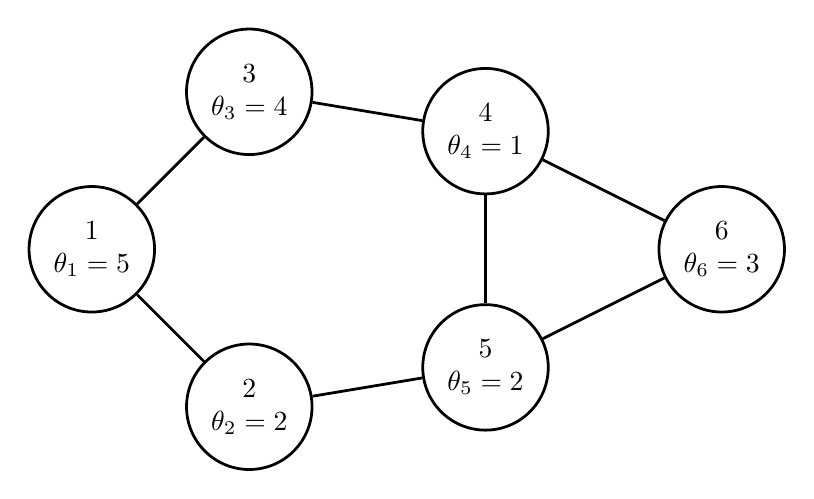
\begin{tikzpicture}[line width=1pt]
        \tikzstyle{every node}=[draw,circle,text width=3em,text badly centered];
        \node (a) at (0,0) {1\\$\theta_1 = 5$};
        \node (x) at (2,-2) {2\\$\theta_2 = 2$};
        \node (z) at (2,2) {3\\$\theta_3 = 4$};
        \node (d) at (5,1.5) {4\\$\theta_4 = 1$};
        \node (b) at (5,-1.5) {5\\$\theta_5 = 2$};
        \node (y) at (8,0) {6\\$\theta_6 = 3$};
        \draw (a) -- (z) -- (d) -- (y) -- (b) -- (x) -- (a);
        \draw (d) -- (b);
      \end{tikzpicture}
    \end{center}
  \end{minipage}
  \caption{Example Inter-domain routing problem. The nodes represent
    networks. Each one shows the cost it would incur in transporting a
    packet through its network. The agents' types are their costs.}
  \label{fig:routing}
\end{SCfigure}

\medskip

Figure~\ref{fig:routing} shows a sample inter-domain routing problem.
In this problem each node represents a computer network. The edges
represent how these networks are connected to each other. Each network
is willing to handle packets whose source or destination address is
within the network. However, they are reticent to carry packets that
are just passing thru. Each network in the figure also shows the cost
it incurs in routing one of these passing-thru packets. These costs
correspond to the agents' types. That is, only the agent knows how
much it costs to pass a packet across its network. We further assume
that we know how much traffic will travel from every start node to
every destination node. The problem then is to find the routes for
each source-destination pair such that the costs are minimized. This
is a mechanism design problem which can be solved in a distributed
manner \cite{feigenbaum05a}, as we now show.

We can formally define the problem as consisting of $n$ agents. Each
agent $i$ knows its cost to be $\theta_i$. An outcome $o$ of our
mechanism design problem corresponds to a set of routing rules for all
source-destination pairs. That is, the outcome $o$ should tell us, for
all $i,j$, which path a packet traveling from $i$ to $j$ should
follow. The value $v_i(o)$ that each agent receives for a particular
outcome $o$ is the negative of the total amount of traffic that $i$
must endure given the paths specified in $o$ and the traffic amounts
between every pair.

The solution we want is then simply
\begin{equation}
  \label{eq:network-scf}
  f(\theta) = \arg \max_{o} \sum_{i} v_i(o).
\end{equation}
Since this is the social-welfare maximizing solution we are free to
use \acro{vcg} payments to solve the problem. Specifically, we can ask
all agents to report their costs $\tilde{\theta}$ and then use
\eqref{eq:vcg-payments} to calculate everyone's payments thus ensuring
that telling the truth is the dominant strategy for all agents. Note
that, in this case, calculating the outcome given $\tilde{\theta}$
amounts to calculating a minimum spanning tree for each destination
node $j$. The problem of finding the routes that minimize the sum of
all costs has already been solved, in a distributed manner, by the
standard Internet \td{Border Gateway Protocol} (\acro{bgp}). The
protocol works by propagating back the minimum costs to a given
destination.  All agents tell each other their costs to destination.
Each agent then updates its cost to a destination by adding its own
transportation costs. The process then repeats until quiescence. The
algorithm is, in fact, a variation on Dijkstra's algorithm for finding
shortest paths in a graph \cite{dijkstra59a}.

Note, however, that the payment calculation \eqref{eq:vcg-payments}
requires us to find the sum of everyone else's valuation for the case
where $i$ does not exist, the second term in \eqref{eq:vcg-payments}.
For this problem, eliminating $i$ simply means eliminating all links
to $i$. But, it could be that the elimination of these links
partitions the graph into two or more pieces thereby making it
impossible for traffic from some nodes to reach other nodes. In such a
case then it would be impossible to calculate the \acro{vcg} payments.
Thus, we must make the further assumption that the network is
\td{bi-connected}: any one node can be eliminated and still every node
can be reached from every other node.

We also note that the \acro{vcg} payments can be broken down into a sum
\begin{equation}
  \label{eq:routing-sum}
  p_i(\tilde{\theta}) = \sum_{a,b} p_i(a,b,\tilde{\theta}), 
\end{equation}
where $p_i(a,b,\tilde{\theta})$ is the payment that $i$ receives for
the traffic that goes from node $a$ to node $b$. This payment can be
further broken down into its constituent \acro{vcg} parts: the value
everyone else gets and the value everyone else would get if $i$ did
not exist.  We can find these by first defining the total cost
incurred in sending a packet from $a$ to $b$. We let
$\id{lowest-cost-path}(a,b,\tilde{\theta})$ be the lowest cost path --
a list of nodes -- for sending a packet from $a$ to $b$ given
$\tilde{\theta}$.  The total cost associated with that path is given
by
\begin{equation}
  \label{eq:cost}
\id{cost}(a,b,\tilde{\theta}) = \sum_{i \in
  \id{lowest-cost-path}(a,b,\tilde{\theta})} \tilde{\theta}_i,
\end{equation}
which is simply the sum of the costs in all the intervening nodes. We
can then determine that the payment that $i$ gets is given by
\begin{equation}
  \label{eq:pay1}
  p_i(a,b,\tilde(\theta)) = \tilde{\theta}_i -
  \id{cost}(a,b,\tilde{\theta}_i) + \id{cost}_{-i}(a,b,\tilde{\theta}_i),
\end{equation}
where $\id{cost}_{-i}(a,b,\tilde{\theta}_i)$ is defined in the same as
\id{cost} but for a graph without agent $i$. Note how this payment
equation is really just the \acro{vcg} payments once again. The first
two terms capture the value that everyone else receives while the
third term capture the value that everyone else receives if $i$ did
not exist; since $i$ does not exist he does not contribute cost. The
main difference is that the signs are reversed since we are dealing
with costs and not value.

We now note that since the payments depend solely on the costs of the
lowest cost path from $i$ to $j$ then some of these costs could be
found by adding other costs. For example, if the lowest cost path from
$i$ to $j$ involves first going from $i$ to $a$ directly and then
taking the lowest cost path from $a$ to $j$ then the
$\id{cost}(i,j,\tilde{\theta}) = \tilde{\theta}_i +
\id{cost}(a,j,\tilde{\theta})$. A careful analysis of these type of
constraints leads us to deduce that for all $k \in
\id{lowest-cost-path}(i,j,\tilde{\theta})$ where $a$ is a neighbor of
$i$, we have that:
\begin{enumerate}
\item If $a$ is $i$'s parent in
  $\id{lowest-cost-path}(i,j,\tilde{\theta})$ then $p_k(i,j) =
  p_k(a,j)$.
\item If $a$ is $i$'s child in
  $\id{lowest-cost-path}(i,j,\tilde{\theta})$ then $p_k(i,j) =
  p_k(a,j) + \tilde{\theta}_i + \tilde{\theta}_a$.
\item If $i$ is neither a parent or a child of $i$ and $k \in
  \id{lowest-cost-path}(a,j,\tilde{\theta})$ then $p_i(i,j) =
  \tilde{\theta}_a + \id{cost}(a,j) = \id{cost}(i,j)$.
\item If $i$ is neither a parent or a child of $i$ and $k \not\in
  \id{lowest-cost-path}(a,j,\tilde{\theta})$ then $p_k(i,j) =
  \tilde{\theta}_k + \tilde{\theta}_a + \id{cost}(a,j) -
  \id{cost}(i,j)$.
\end{enumerate}

\begin{SCfigure}
  \begin{minipage}{1.0\linewidth}
    \begin{codebox}
      \Procname{$\proc{initialize}()$}
      \li \For $j \gets 1\ldots n$ \Comment for each destination $j$
      \li \Do calculate $\id{lowest-cost-path}(i,j)$
      and $\id{cost}(i,j)$
      \li   \For $k \in \id{lowest-cost-path}(i,j)$
      \li     \Do $p_k[i,j] \gets \infty$
              \End
          \End
    \end{codebox}
    \begin{codebox}
      \Procname{$\proc{handle-update}(a, j, \id{cost-aj}, \id{path}, \id{payments})$}
      \zi \Comment $a$ is the agent sending the message (invoking this
      procedure).
      \zi \Comment $j$ is the destination node.
      \zi \Comment \id{cost-aj} is the reported cost of sending a packet
      from $a$ to $j$.
      \zi \Comment \id{path} is a list of nodes on the lowest cost
      path from $a$ to $j$.
      \zi \Comment \id{payments} are the payments for each node on
      \id{path}.
      \li $\id{modified} \gets \const{false}$
      \li \If $a \in \id{lowest-cost-path}(i,j)$ \Comment Parent
      \li \Then \For $k \in \id{path}$
      \li       \Do \If $p_k[i,j] > p_k[a,j]$
      \li           \Then $p_k[i,j] \gets p_k[a,j]$
      \li                 $\id{modified} \gets \const{true}$
                    \End
                \End
      \li \ElseIf $i \in \id{lowest-cost-path}(a,j)$ \Comment Child
      \li \Then \For $k \in $ \{All but last item in \id{path}\}
      \li       \Do \If $p_k[i,j] > p_k[a,j] + \tilde{\theta}_a + \tilde{\theta}_i$
      \li           \Then $p_k[i,j] \gets p_k[a,j] + \tilde{\theta}_a
      + \tilde{\theta}_i$
      \li                 $\id{modified} \gets \const{true}$
                    \End
                \End
      \li \ElseNoIf 
      \li $t \gets $ position of last node for which \id{path}
      equals $\id{lowest-cost-path}(i,j)$
      \li     \For $k \in \id{lowest-cost-path}(i,j)[1\twodots t]$
      \li     \Do \If $p_k[i,j] > p_k[a,j] + \tilde{\theta}_a +
      \id{cost-aj} - \id{cost}(i,j)$
      \li         \Then $p_k[i,j] \gets p_k[a,j] + \tilde{\theta}_a +
      \id{cost-aj} - \id{cost}(i,j)$
      \li               $\id{modified} \gets \const{true}$
                  \End
              \End
      \li     \For $k \in \id{lowest-cost-path}(i,j)[t+1\twodots]$

      \li     \Do \If $p_k[i,j] > \tilde{\theta}_k + \tilde{\theta}_a
      + \id{cost-aj} - \id{cost}(i,j)$
      \li         \Then $p_k[i,j] \gets \tilde{\theta}_k + \tilde{\theta}_a
      + \id{cost-aj} - \id{cost}(i,j)$
      \li               $\id{modified} \gets \const{true}$
                  \End
              \End
          \End
      \li \If \id{modified} 
      \li \Then $\id{my-payments} \gets p_k[i,j]$ for $k \in
      \id{lowest-cost-path}(i,j)$ 
      \li       \For $b$ is my neighbor
      \li       \Do $b.\proc{handle-update}(i,j,\id{cost}(i,j),$
      \zi \>\>\>$\id{lowest-cost-path}[i,j], \id{my-payments})$
                \End
          \End
    \end{codebox}
    \caption{Algorithm for calculating \acro{vcg} payments for the
      inter-domain routing problem. $i$ refers to the agent running the
      algorithm. All agents start by executing \proc{initialize} and
      then send a \proc{handle-update} to all their neighbors.}
    \label{fig:vcg-routing-alg}
  \end{minipage}
\end{SCfigure}
We can then build an algorithm where the agents send each other
payment tables and then update their own payment tables using the ones
they received along with the above equations.
Figure~\ref{fig:vcg-routing-alg} shows such an algorithm. All agents
start by executing the procedure \proc{initialize} and then send
\proc{handle-update} to their neighbors in order to get the process
going. The algorithm has been shown to converge to the true prices for
agents.

Note that the calculation of \id{lowest-cost-path} is itself a
distributed calculation that is being carried out simultaneously by
the \acro{bgp} algorithm.  This means that the values of
\id{lowest-cost-path} are also changing and, thus, might be incorrect.
However, it has been shown that the payment calculations will converge
even in the presence of such changes.


\subsection{Mechanism Design Summary}

Mechanism design provides us with a solid mathematical framework for
expressing many multiagent design problems. Specifically, we can
represent problems involving selfish agents who are intelligent enough
to lie if it will increase their utility. Furthermore, the
Groves-Clarke and \acro{vcg} payment equations give us a ready-made solution
for these problems. Unfortunately, this solution only works if we can
implements payments and, even then, the payments are not
revenue-neutral so we need an infinite amount of cash to give the
agents. Also, these solutions are centralized in that all types are
reported to a central agent who is then in charge of calculating and
distributing the payments.

Distributed mechanism design is a new research area: few effective
algorithms exist and many roadblocks are visible. Different approaches
are being taken to overcome these roadblocks. One approach is to
extend the mechanism design problem by defining trust-based mechanisms
in which agents take into account the degree of trust they have on
each other when determining their allocations \cite{dash04a}. Another
approach is to distribute the calculation of \acro{vcg} payments by
using redundantly asking agents to perform sub-problems
\cite{parkes04a} and use encryption \cite{monderer99a}.


%\subsection{Recent Advances in Mechanism Design}
%Feigenbaums' class
%http://zoo.cs.yale.edu/classes/cs455/

%Parkes has papers on detecting un-faithfulness in bittorrent
%Also check out his class
%http://www.eecs.harvard.edu/~parkes/cs286r/spring05/schedule.html for
%more papers.
%http://www.eecs.harvard.edu/~parkes/cs286r/spring06/schedule.html

% \cite{larson05a} have looked at mechanism design using deliberative
% agents. They define deliberative agents as those that do not have a
% priori knowledge of their $v_i$ function an must instead computer them
% as needed or gather information needed to compute them. In their words
% ``A deliberative agent is an agent who must compute or gather
% information in order to determine its preferences, has restrictions on
% its computing or information gathering capabilities, and who carefully
% considers how to use its available resources given its restrictions.''
% They give new definitions for desirable mechanism and then show how
% these are impossible---all negative results thus far.

% \section{History}
% \label{sec:history-1}

% \cite{varian95a} was one of the first to propose the use of mechanism
% design for building multiagent systems.

% \cite{feigenbaum02a} is a good summary paper listing the most
% important results in \acro{damd} in general and, specifically, as they
% pertain to network routing, overlay networks, and P2P file sharing
% problems. Finally, \cite{dash03a} is another introduction to mechanism
% design and distributed mechanism design.




%%% Local Variables: 
%%% mode: latex
%%% TeX-master: "~/wp/mas/mas"
%%% TeX-command-default: "PDFlatex"
%%% End:
